\documentclass[a4paper,12pt]{article}
\usepackage{amssymb}
\usepackage{amsmath}
\usepackage{hhline}
\usepackage{ragged2e}
\usepackage{physics}
\usepackage{bm}
\usepackage[margin=2cm]{geometry}
\usepackage{bigfoot}
\usepackage{amsthm}
\usepackage{tikz}
\usepackage{tabularx}
\usepackage{graphicx}
\usetikzlibrary{shapes.geometric, arrows}
\tikzstyle{startstop} = [rectangle, rounded corners, minimum width=3cm, minimum height=1cm,text centered, draw=black, fill=red!30]
\tikzstyle{io} = [trapezium, trapezium left angle=70, trapezium right angle=110, minimum width=3cm, minimum height=1cm, text centered, draw=black, fill=blue!30]
\tikzstyle{process} = [rectangle, minimum width=3cm, minimum height=1cm, text centered, draw=black, fill=orange!30]
\tikzstyle{decision} = [diamond,aspect = 2, text centered, draw=black, fill=green!30]
\tikzstyle{arrow} = [thick,->,>=stealth]
\usepackage{newunicodechar}
\newunicodechar{≠}{\ensuremath{\not =}}
\usepackage{textcomp}
\usepackage[makeroom]{cancel}

\newlength\mylength
\setlength\mylength{0.1cm}
\newcolumntype{Y}{>{\Centering\arraybackslash}X}

\newtheoremstyle{break}
  {\partopsep}{\topsep}%  
  {\normalfont}{}
  {\bfseries}{}%
  {\newline}{}%
  \theoremstyle{break}
\newtheorem{theorem}{Teorema}[section]
\newtheorem{corollary}{Corollario}[section]
\newtheorem{proposition}{Proposizione}[section]
\renewcommand*{\proofname}{\textbf{Dimostrazione}}
\renewcommand\qedsymbol{$\bigstar$}
\newtheorem{definition}{Definizione}[section]

\let\oldemptyset\emptyset
\let\emptyset\varnothing

\newcommand{\ind}{\perp\!\!\!\!\perp} 
\newcommand{\code}[1]{\texttt{#1}}
\newcommand{\xdownarrow}[1]{%
  {\left\downarrow\vbox to #1{}\right.\kern-\nulldelimiterspace}
}
\newcommand{\xuparrow}[1]{%
  {\left\uparrow\vbox to #1{}\right.\kern-\nulldelimiterspace}
}
\newcommand{\arrvline}{\hfil\kern\arraycolsep\vline\kern-\arraycolsep\hfilneg}

\long\def\symbolfootnotemark[#1]#2{\begingroup%
\def\thefootnote{\fnsymbol{footnote}}\footnotetext[#1]{#2}\footnotemark[#1]\endgroup}

\long\def\symbolfootnotetext[#1]#2{\begingroup%
\def\thefootnote{\fnsymbol{footnote}}\footnotetext[#1]{#2}\endgroup}


\numberwithin{equation}{section}





\begin{document}
\title{Appunti di Algoritmi e Architetture per il Calcolo ad Alte Prestazioni}
\author{Andrea Bonifacio}
\date{\today}
\maketitle
\newpage
\section{Architettura dei Calcolatori}
\subsection{Introduzione}
I computer sono il prodotto di una industria nuova e in continuo cambiamento. Negli ultimi 30 anni il paradigma fondamentale di questa continua innvovazione era stato dato dalla Legge di Moore
\begin{quote}
    ``La complessità di un microcircuito, misurata ad esempio tramite il numero di transistor per chip, raddoppia ogni 18 mesi (e quadruplica quindi ogni 3 anni).'' 
\end{quote}
Dai loro albori a oggi i computer hanno fatto tantissima strada, al giorno d'oggi si trovano in quasi ogni oggetto presente nella vita delle persone
\begin{itemize}
    \item Automobili: ormai praticamente tutto ciò che è presente nelle automobili è governato da un microprocessore, questo è avvenuto grazie al rapido miglioramento di questi ultimi sia dal punto di vista economico che delle prestazioni.
    \item Cellulari: negli ultimi venti anni sono diventati parte integrante della vita di tutti i giorni.
    \item Humane Genome Project: il continuo diminuire del prezzo dei singoli computer a parità di prestazioni ha permesso la creazione di questo enorme progetto per sequenziare tutto il genoma umano.
    \item World Wide Web: senza aggiungere altro, forse la più grande rivoluzione del terzo millennio.
\end{itemize}
Esistono varie categorie di calcolatori, sicuramente le principali in cui si possono suddividere sono:
\begin{itemize}
    \item Personal Computer (PC): macchine per il singolo operatore che permettono di avere un buon compromesso tra prezzo e prestazioni.
    \item Server: macchine pensate per un utilizzo costante, spesso da una serie di operatori diversi. Esistono server che si occupano di algoritmi complessi e server che eseguono semplici compiti continuamente. In termini di spazio e costi, non sono ben definibili, possono avere le dimensioni e i prezzi di un normale PC, oppure costare svariate decine di migliaia di Euro e occupare una intera stanza.
    \item Embedded computer\footnote{Non riesco a pensare a una traduzione migliore}: la classe più ampia, in quanto spaziano dai microprocessori dentro le automobili al network di processori che gestiscono vari sistemi dentro un aeroplano. I sistemi embedded sono generalmente progettati per far girare una singola applicazione.
\end{itemize}
\subsection{Otto idee fondamentali nell'architettura dei computer}
Nella storia della progettazione dei computer, ci sono state otto intuizioni che sono riuscite a perdurare nel tempo, anni e anni dopo la loro formulazione. Nello specifico si tratta di:
\begin{enumerate}
    \item Progettare seguendo la legge di Moore: in quanto il cambiamento continuo è sempre stato una costante all'interno dell'industria IT, era necessario per i vari progettisti rendersi conto di dove sarebbe arrivata la tecnologia al momento del lancio del loro prodotto.
    \item Astrazione: per semplificarsi il lavoro, è stato necessario lavorare con vari livelli di astrazione, non più partendo dal singolo transistor, per salire nei vari livelli, ma creando un sistema astratto per modellizzarli.
    \item Rendere veloce il Common Case: concentrarsi sul rendere veloci le operazioni basiche, senza concentrarsi su come rendere performanti le operazioni meno comuni, permette di ottimizzare in maniera molto più semplice.
    \item Parallelizzazione: già dai primi computer il principale obbiettivo era raggiungere in maniera efficiente l'esecuzione di istruzioni in parallelo, in quanto permetteva di ridurre di parecchio il tempo di esecuzione e aumentare le prestazioni del sistema.
    \item Pipelining: tra gli esempi di parallelzzazione si trova il pipelining, che permette, agendo sostanzialmente come una catena di montaggio, dove ogni elemento esegue un singolo compito e poi passa il testimone all'elemento dopo per eseguire il compito successivo, mentre lui continua a eseguire il suo.
    \item Predizione: la tecnica di eseguire in anticipo operazioni che, probabilmente, verranno richieste a breve per ridurre i tempi. Ovviamente in questo caso serve un meccanismo di recupero in caso di predizione errata e stare attenti a non sbagliare troppo le predizioni.
    \item Gerarchia delle memorie: per accedere ai dati velocemente è necessario avere memorie veloci e molto costose, quindi tendenzialmente si usano memorie piccole per contenere i costi, mentre memorie più grandi e meno costose saranno più lente. Si tende quindi a gerarchizzare le memorie, in maniera da accedere prima alle memorie più veloci e poi a scendere.
    \item Disponibilità: forse meno interessante all'utente finale, ma sicuramente fondamentale per i progettisti di server, oltre a essere veloci, devono essere affidabili e disponibili, per cui si tende ad avere magari più elementi che eseguono lo stesso compito, in maniera che il malfunzionamento di uno di essi non comprometta l'integrità dell'intero sistema.
\end{enumerate}
\subsection{Funzionamento di un programma}
Un normale programma, come può esserlo un editor di testo, arriva a essere formato da milioni di righe di codice, che a loro volta vanno tradotte in linguaggio macchina. Per fare ciò si utilizza in gran parte l'astrazione. Sostanzialmente ci sono tre livelli fondamentali:
\begin{enumerate}
    \item Applicazione o programma: il livello più esterno e "vicino" all'utente.
    \item Software di sistema: tutto quell'insieme di componenti che permettono al programma di interfacciarsi con l'hardware
    \item Hardware: la parte fisica, il 'bare metal' della macchina.
\end{enumerate}
Perché un computer possa interpretare le istruzioni di un programma deve ricevere delle istruzioni ben specifiche da mandare al processore. Chiaramente non è il modo più comodo di lavorare, in quanto questi linguaggi macchina sono spesso complicati e poco intuitivi da scrivere. Si ricorre allora all'utilizzo di linguaggi di alto livello (HLL), che sono più comprensibili all'occhio umano. Il passaggio da HLL a linguaggio di basso livello (LLL) avviene tramite un compilatore, un programma che è in grado di tradurre il linguaggio di alto livello nel codice macchina corretto del processore.
\subsection{Dentro a un computer}
Nell'informatica classica, una delle definizioni accettate di computer è quella di Von Neumann, dove sono presenti i dispositivi di input (mouse, tastiera, microfoni), quelli di output (schermi, altoparlanti), la memoria e il processore, che sono sostanzialmente gli elementi minimi necessari per far funzionare un computer. 


Tra gli elementi di output il più noto è sicuramente lo schermo. La maggior parte di essi funziona con la tecnologia a cristalli liquidi (LCD), che è sostanzialmente una matrice di cristalli che vengono illuminati secondo le quantità di colore RGB necessarie per creare l'immagine richiesta. Il computer ha una matrice di dati, detta frame buffer che contiene le informazioni in codice binario che compongono l'immagine che verrà poi tradotta dal monitor. 


Sovrapponendo a un LCD un pannello capacitivo che permette di determinare la posizione del tocco dell'utente e si ottiene un touchscreen.


All'interno di tutti i computer si trovano i circuiti integrati, detti anche chip, che possono avere diversi compiti, dal processore principale (CPU) ai vari controller di dispositivi all'interno del computer. 
Per tornare al discorso dell'astrazione, uno dei passaggi fondamentali nella progettazione di un computer è la scelta di un set di istruzioni (ISA) per un determinato processore. Un ISA è il minimo necessario per poter interfacciarsi con il processore senza dover scrivere codice binario.
Un circuito integrato solitamente è formato da una serie di transistor, che altro non sono che degli switch on-off che cambiano stato se attraversati da corrente. La crescita del numero di transistor presenti all'interno di un chip è stata quasi esponenziale, come ricorda la legge di Moore. Il silicio, come altri elementi simili è un semiconduttore, per cui ha sia caratteristiche di un conduttore che di un isolante, a seconda di come viene trattato o delle temperature a cui opera. 


Per ottenere un chip si parte da un lingotto di silicio, che viene diviso in tante fette rotonde (dette wafer), sopra le quali viene impresso e lavorato il circuito mediante complicati processi industriali\footnote{Credetemi, ci ho lavorato dentro, complicato non rende l'idea}. Una volta ottenuto un wafer con sopra una serie di chip uguali vengono tagliati e testati per il funzionamento. Dopo questo passaggio sono pronti per essere venduti o installati dentro dei componenti.
Questo processo di produzione in serie permette di scartare solo pochi chip.
Il costo di produzione di un circuito integrato si ottiene con una serie di equazioni.
\begin{gather*}
    \mbox{Costo per chip}=\frac{\mbox{Costo per wafer}}{\mbox{Chip per wafer} \times \mbox{Rendimento}} \\
    \mbox{Chip per wafer} \approx \frac{\mbox{Area del wafer}}{\mbox{Area del chip}} \\
    \mbox{Rendimento} = \frac{1}{(1 + (\mbox{Difetti per area} \times \mbox{Area del chip}))^2}
\end{gather*}
L'ultima equazione è ottenuta da una serie di dati empirici ottenuti da varie fabbriche di chip, l'esponente tendenzialmente è legato al numero di step critici all'interno del processo produttivo.
\subsection{Prestazioni}
Un altro problema presente dagli albori di queste nuove tecnologie è sempre stato quello di definire in maniera corretta le prestazioni di un sistema. Ha più senso un sistema in grado di eseguire \(n\) operazioni al secondo ma che consuma una energia pari a \(m\), o un sistema che ne esegue \(\frac{n}{10}\), ma consuma \(\frac{m}{100}\) energia? Parecchie persone hanno pensato a questa questione, e sono giunti a due principali metriche in grado di fare dei confronti sensati tra vari sistemi.
Si tratta di 
\begin{enumerate}
    \item Latenza o tempo di risposta: probabilmente la più intuibile, determina il tempo in cui un sistema risponde a un determinato input.
    \item Portata: il numero di operazioni eseguite da un sistema in un determinato lasso di tempo.
\end{enumerate}
tendenzialmente per sistemi customer-oriented si osserva più la latenza, in quanto può essere anche un punto di forza in caso di vendita, mentre se si tratta di grossi sistemi di server la portata sarà una metrica più utile, in quanto si vorrà massimizzare la quantità di operazioni al secondo.


Nell'ambito della comparazione tra prestazioni, si supponga di voler confrontare un sistema \(X\) e un sistema \(Y\), si definiscano le prestazioni come 
\[
    \mbox{Prestazioni} = \frac{1}{\mbox{Tempo di risposta}}
\]
Allora se le prestazioni di \(X\) sono migliori delle prestazioni di \(Y\) vuol dire che 
\begin{gather*}
    \mbox{Prestazioni}_X > \mbox{Prestazioni}_Y \\
    \frac{1}{\mbox{Tempo di risposta}_X} > \frac{1}{\mbox{Tempo di risposta}_Y} \\
    \mbox{Tempo di risposta}_Y > \mbox{Tempo di risposta}_X
\end{gather*}
Allora si può anche ottenere un numero \(n\) definito come 
\[
    \frac{\mbox{Prestazioni}_X}{\mbox{Prestazioni}_Y} = n
\]
In tal modo si può dire che il sistema \(X\) è \(n\) volte più veloce di \(Y\). 


Nel caso dei computer il tempo di risposta è spesso correlato al tempo di lavoro della CPU. Per misurare il tempo di utilizzo di una CPU si ricorre all'utilizzo di un 'orologio' interno che definisce il tempo in cui avvengono gli eventi nel sistema. Tale orologio si definisce clock cycle, generalmente ha valori di parecchi ordini di grandezza più piccoli dei secondi, in quanto le operazioni all'interno del processore avvengono con velocità impressionante. Allora invece del periodo di clock, spesso si utilizza il suo inverso, la frequenza di clock, che indica quanti cicli vengono completati in un secondo. 


Allora si può definire il tempo di esecuzione di un programma come 
\begin{align*}
    \mbox{Tempo di esecuzione della CPU 
    di un programma} = \mbox{Cicli di clock per eseguire il programma}  \\
    \times \quad \mbox{Tempo di un singolo ciclo}
\end{align*}
\begin{gather*}
    \mbox{Tempo di esecuzione della CPU di un programma} = \frac{\mbox{Cicli di clock per eseguire il programma}}{\mbox{Frequenza di clock}}
\end{gather*}
Tuttavia queste metriche sono molto approssimative e non tengono conto di svariati fattori, uno fra tutti quante istruzioni vengono eseguite durante l'esecuzione del programma. Si può parlare allora di cicli di clock della CPU come 
\begin{align*}
    \mbox{Cicli di clock della CPU} = \mbox{Numero di istruzioni per il programma} \\ \times \quad \mbox{Numero medio di cicli di clock per istruzione}
\end{align*}
Il termine \textit{Numero medio di cicli di clock per istruzione} si chiama anche cicli di clock per istruzione (CPI) ed è una comoda metrica che permette di definire il tempo CPU come
\[
    \mbox{Tempo CPU} = \frac{\mbox{Numero di istruzioni} \times \; \mbox{CPI}}{\mbox{Frequenza di clock}}
\]
Ci sono quindi vari modi per definire le prestazioni di un sistema, e si può agire sulle singole metriche per migliorare il sistema, ma bisogna sempre tenere conto dell'efficienza del sistema.
\subsection{La questione energetica}
Negli ultimi decenni ci si è resi conto di aver raggiunto un limite fisico al raffreddamento dei processori, per cui non possono assorbere più di una determinata potenza. Oltretutto con il proliferare di dispositivi alimentati da batterie e non connessi a una sorgente continua di elettricità si è dovuto cercare un giusto compromesso tra energia consumata e prestazioni. 
Poiché si era giunti alla conclusione che il consumo di potenza si poteva calcolare come 
\[
    \mbox{Potenza} \propto \frac{1}{2} \; \times \; \mbox{Carico capacitivo} \; \times \; \mbox{Tensione}^2 \; \times \; \mbox{Frequenza}
\]
Poiché le frequenze sono aumentate di mille volte negli ultimi 30 anni e la tensione è arrivata da \(5V\) a \(1V\), ci si aspetterebbe un incremento della potenza notevole, mentre si parla di un aumento di circa trenta volte dagli anni '80. Purtroppo la tensione ha raggiunto un livello fisico insuperabile e la frequenza si è stabilizzata ormai, dunque si è raggiunto un tetto massimo alla potenza assorbita dai chip.
Incapaci di trovare una soluzione pratica al problema energetico, i progettisti hanno utilizzato la soluzione temporanea di aumentare il numero di \textit{cores} di un processore, arrivando ad avere magari otto unità dentro un singolo processore che potessero lavorare separatamente. 


La questione dell'ottimizzazione energetica ha inoltre portato alla luce una serie di fallacie o problematiche che impediscono il progredire come era successo nelle ultime decadi
\begin{itemize}
    \item Legge di Amdahl: si può riassumere come \begin{quote}
        Il miglioramento che si può ottenere su una certa parte del sistema è limitato dalla frazione di tempo in cui tale attività ha luogo.
    \end{quote}
    Ossia che a volte lavorare per migliorare una singola porzione di un sistema rischia di non produrre nessun effetto utile, ad esempio nel caso in cui tale operazione sia già stata ottimizzata al massimo. Si può formulare come 
    \begin{align*}
        \mbox{Tempo di esecuzione dopo il miglioramento} = \\
        \frac{\mbox{Tempo di esecuzione influenzato dal miglioramento}}{\# \;\mbox{di volte che è migliorato il processo}} \; + \\
        + \; \mbox{Tempo di esecuzione non influenzato}
    \end{align*}
    Si può utilizzare tale legge per stimare il miglioramento delle prestazion di un sistema conoscendo il tempo speso a fare determinati compiti e il miglioramento potenziale.
    \item Consumo di energia al minimo: non si è ancora trovata una soluzione al rendere il consumo di energia lineare al carico di lavoro. Anche i sistemi più ottimizzati al \(10\%\) del carico di lavoro consumano il \(33\%\) della potenza massima.
    \item Utilizzare un elemento solo dell'equazione delle prestazioni come metrica: una alternativa al tempo di esecuzione sono le MIPS (Million Instructions Per Second) definita come 
    \[
        \mbox{MIPS} = \frac{\mbox{Numero di istruzioni}}{\mbox{Tempo di esecuzione} \; \times \; 10^6}
    \]
    I problemi di questa metrica sono principalmente tre, in primo luogo non tiene conto dei diversi set di istruzioni e le loro velocità, inoltre varia da programma a programma sullo stesso computer, e inoltre in un programma con più istruzioni, ma la singola istruzione è più veloce, le MIPS variano indipendentemente dalle prestazioni.
\end{itemize}
\newpage
\section{Istruzioni: il linguaggio dei computer}
\subsection{Introduzione}
Interagire con l'hardware di un computer, come detto in precedenza, richiede l'utilizzo di un set di istruzioni. Generalmente quando si parla di set di istruzioni si parla di linguaggi tutto sommato simili tra di loro, con delle filosofie alla base molto differenti. In questo caso il linguaggio in uso sarà il RISC-V, ma ne esistono molte altre, tra le più note Intel x86, MIPS e ARM.
\subsection{Operazioni}
Ogni computer è in grado di eseguire calcoli aritmetici. Nel caso del RISC-V il codice per sommare due numeri è dato da
\begin{verbatim}
    add a, b ,c
\end{verbatim}
che richiede al computer di sommare i numeri \code{b} e \code{c} e di salvare tale somma in \code{a}.
Si tratta di un comando molto rigido che ha sempre una sola variabile come output e ne accetta due come input, per cui per sommare tra di loro quattro variabili diverse è necessario 
\begin{verbatim}
    add a, x, y             // La somma di x e y si trova in a
    add a, a, w             // La somma di x, y e w si trova in a
    add a, a, z             // La somma di x, y, w, e z si trova in a
\end{verbatim}
Tutte le parole oltre il doppio slash sono commenti che vengono ignorati e servono solo al lettore umano. 


Questa scelta deriva da una filosofia di progettazione, la semplicità favorisce la regolarità. Tante operazioni semplici ripetute spesso rendono più veloce e regolare il flusso di lavoro.
Per esempio un programma più complesso\footnote{Ho visto programmi più complicati} in C come può essere 
\begin{verbatim}
    f = (g + h) - (i + j);
\end{verbatim}
che contiene 5 variabili\footnote{Lo so, andavano dichiarate prima perdonatemi} \code{f, g, h, i, j} viene tradotto nel seguente modo da un compilatore C \(\to\) RISC-V
\begin{verbatim}
    add t0, g, h            // Crea una variabile temporanea per la somma 
                            di g e h
    add t1, i, j            // Variabile temporanea per i e j
    sub f, t0, t1           // Salva in f la differenza delle due variabili 
                            temporanee
\end{verbatim}
\subsection{Operandi}
Gli operandi per eseguire istruzioni aritmetiche sono salvati all'interno di determinati registri del RISC-V. Un registro è un insieme di \(64\) bit all'interno dell'hardware. Poiché appaiono molto spesso, i gruppi di \(64\) bit sono definiti \textit{doublewords}, mentre i gruppi di \(32\) bit sono chiamati \textit{words}. A differenza delle variabili di un linguaggio di programmazione, il numero di registri in un set di istruzioni è limitato, in questo caso a \(32\) registri.
Tale limite nasce da una seconda scelta stilistica: più una cosa è piccola più è veloce. Minore è il numero di registri da controllare, minore sarà il tempo di clock.  

I \(32\) registri hanno tutti delle funzioni specifiche
\begin{itemize}
    \item \code{x0}: la costante nulla
    \item \code{x1}: indirizzo di return
    \item \code{x2}: puntatore dello stack
    \item \code{x3}: puntatore globale
    \item \code{x4}: puntatore del thread
    \item \code{x5} - \code{x7}, \code{28} - \code{x31}: temporanee
    \item \code{x8}: puntatore del frame
    \item \code{x9}, \code{18} - \code{x27}: salvataggio variabili
    \item \code{x10} - \code{x11}: argomento funzioni/risultato
    \item \code{x12} - \code{x17}: argomento funzioni
\end{itemize}

Poiché il numero di registri è limitato, è necessario avere un posto dove salvare i dati che non servono nell'immediato futuro. Ci sono delle istruzioni apposta per trasferire i dati dai registri alla memoria. La memoria è strutturata come un singolo vettore monodimensionale, a cui si accede utilizzando l'indirizzo della cella interessata. 

L'istruzione per trasferire i dati in memoria generalmente si chiama \textit{load} e ha una sintassi per cui prende come input la variabile da salvare, la cella dove salvarla e una costante che rappresenta la memoria. Nel caso del RISC-V il comando è dato da \code{ld}. 

Supponendo di voler caricare nell'array memoria le variabili \code{g} e \code{i}, sia l'array memoria definito come \code{A} per comodità. Osservando questo snippet di codice C
\begin{verbatim}
    g = h + A[8]
\end{verbatim}
Nonostante si tratti di una singola operazione, è necessario prima estrarre il valore \code{A[8]}, e per farlo si utilizza proprio il comando \code{ld}.
Il comando \code{ld} carica il valore di \code{A[8]} in un registro temporaneo, in questo caso \code{x9}. Il valore \code{h} è salvato nel registro \code{x21} e il valore \code{g} in \code{x20}. Per accedere alla memoria \code{A} bisogna prendere il primo elemento, che si trova in \code{x22} e sommare la costante \code{8}

Il codice prodotto dal compilatore sarà del tipo:
\begin{verbatim}
    ld x9, 64(x22)        // Il valore di A[8] viene caricato in x9
    add x20, x21, x9      // g = h + A[8]
\end{verbatim}
Il comando \code{8(x22)} prende il registro base dall'indirizzo \code{x22} e aggiunge un offset di \code{8}, che va moltiplicato per \(8\), essendo un byte composto da \(8\) singoli bit.
Il comando che esegue il compito opposto, ossia carica dei dati da un registro alla memoria è detto \code{sd}, che sta per \textit{store doubleword}. 

Nel caso si volesse prendere un valore da un array, sommargli una costante e salvarlo in una nuova posizione all'interno dello stesso array, si dovrebbe scrivere in C
\begin{verbatim}
    A[12] = h + A[8]
\end{verbatim}
Quando viene dato in pasto al compilatore il risultato apparirà simile a:
\begin{verbatim}
    ld x9, 64(x22)
    add x9, x21, x9
    sd x9, 96(x22)
\end{verbatim}
Poiché il valore va salvato nella posizione \(12\) dell'array, il compilatore deve aggiungere un offset di \(8 \times 12\).

Spesso si utilizzano delle costanti nei programmi per determinati compiti, in quel caso si possono utilizzare le costanti immediatamente senza doverle recuperare dalla memoria. 
\begin{verbatim}
    addi x22, x22, 4       // Al valore x22 viene aggiunto un valore costante   
\end{verbatim}
La costante \code{0} è salvata in un registro apposta in quanto viene utilizzata molto spesso. Ad esempio quando si rende negativo un numero si utilizza il comando \code{sub} con la costante \code{0} e il numero da invertire.
\subsection{Numeri interi \textit{signed} e \textit{unsigned}}
Come visto in precedenza, i processori sono formati da svariati transistor, i quali sono come degli switch on/off, per cui possono assumere solo lo stato \(1\) e \(0\). Per tale motivo i computer elaborano i numeri in base binaria.
Una regola generale per convertire un numero da una base non decimale a quella decimale è di suddividere il numero nelle singole cifre \(k_i\) con \(i\) che va da \(0\) alle \(n-1\) cifre del numero e poi eseguire una sommatoria
\[
    \sum_{i=0}^{n-1} k_i \times \mbox{Base}^i
\]
Al contrario invece è necessario prendere il numero in base decimale e dividerlo quante più volte si riesce usando come divisore la base scelta. Risulterà una serie di resti, da \(0\) a \(\mbox{Base}-1\) come valori, e andranno presi dall'ultima divisione effettuata a salire per formare il numero
\begin{center}
    \begin{tabular}{|c|c|c|c|}
    \hline
    Dividendo & Divisore& Risultato & Resto \\
    \(145\) & \(4\) & \(36\) & \(1\) \\
    \(36\) & \(4\) & \(9\) & \(0\) \\
    \(9\) & \(4\) & \(2\) & \(1\) \\
    \(2\) & \(4\) & \(0\) & \(2\) \\
    \hline
    \end{tabular}
   \( \xuparrow{1cm}\)
\end{center}
Si ottiene così che \(145_{10} = 2101_{4}\)

Una doubleword è composta da \(64\) bit, i quali sono numerati da destra verso sinistra. Si parla quindi di bit più significativo per riferirsi al bit più a sinistra (il \(63\)) e di bit meno significativo per il bit più a destra (lo \(0\)). 
Dal momento che una doubleword ha queste dimensioni, è possibile ottenere \(2^{64}\) combinazioni diverse di bit, per un totale di numeri da \(0\) a \(2^{64}-1 \; (18,446,774,074,709,551,615_{10})\).
Tuttavia i numeri rappresentati sono tutti positivi, o meglio, vengono detti \textit{unsigned}. Per rappresentare i numeri negativi si è deciso di prendere il bit più significativo e trasformarlo in un bit di segno, per cui se il numero inzia con uno \(0\) è un numero positivo, altrimenti è un numero negativo. Questo meccanismo è chiamato \textit{complemento a due}.
In tale modo si ottiene la formula per la conversione dei numeri in complemento a due 
\[
    (x_{63} \times -2^{63}) + (x_{62} \times 2^{62}) + (x_{61} \times 2^{61}) + \cdots + (x_1 \times 2^1) + (x_0 \times 2^0)
\]
Il bit di segno viene moltiplicato per \(-2^{63}\) e tutto il resto viene sommato a quel risultato. Il negativo di un numero in complemento a due si ottiene in maniera molto semplice, si prende il numero in base binaria, si invertono tutti gli \(0\) con gli \(1\) e viceversa, e alla fine si somma un \(1\). Esempio: 
\[
\begin{array}{rcc}
     \\
    25 & = &0000000000000000000000000000000000000000000000000000000000011001  \\
    \Downarrow &  &\Downarrow  \\
    -25 & = &1111111111111111111111111111111111111111111111111111111111100111 
\end{array}
\]
\subsection{Rappresentare le istruzioni}
A questo punto si può osservare come i computer leggono le istruzioni che ricevono, visto che comprendono solo il codice binario. Un esempio visto in precedenza era il codice 
\begin{verbatim}
    add x9, x20, x21
\end{verbatim}
che viene rappresentato in base decimale come 
\[
\begin{tabular}{|c|c|c|c|c|c|}
    \hline 
    0 & 21 & 20 & 9 & 0 & 51 \\
    \hline
\end{tabular}
\]
e in base binaria come 
\[
\begin{tabular}{|c|c|c|c|c|c|}
    \hline 
    0000000  & 10101  & 10100  & 000  & 01001 & 0110011 \\
    \hline
    \multicolumn{1}{c}{7 bit} & \multicolumn{1}{c}{5 bit} & \multicolumn{1}{c}{5 bit} & \multicolumn{1}{c}{3 bit} & \multicolumn{1}{c}{5 bit} & \multicolumn{1}{c}{7 bit}
\end{tabular}
\]
Il primo, il quarto e il sesto campo della istruzione in tabella (quelli contenenti \(0, 0, 51\)), assieme dicono al computer RISC-V di compiere una addizione con gli argomenti nei restanti campi. 

Questo layout è detto formato dell'istruzione, e la sua traduzione in codice binario è detta linguaggio macchina. Come si vede dalla somma dei bit presenti nella tabella, le istruzioni in RISC-V sono word da \(32\) bit. Per evitare di scrivere lunghe istruzioni in codice binario si ricorre a un'altra base numerica molto comoda, quella esadecimale. Dal momento che la base \(16\) è una potenza di \(2\), si possono trovare delle corrispondenze tra i singoli valori esadecimali e dei gruppi di \(4\) bit in base \(2\)
\begin{center}
    \[
    \begin{tabular}{|c|c|}
        \hline
        Esadecimale & Binario \\
        \hline 
        0 & 0000 \\
        \hline
        1 & 0001 \\
        \hline
        2 & 0010 \\
        \hline
        3 & 0011 \\
        \hline
        4 & 0100 \\
        \hline
        5 & 0101 \\
        \hline
        6 & 0110 \\
        \hline
        7 & 0111 \\
        \hline
        8 & 1000 \\
        \hline
        9 & 1001 \\
        \hline
        a & 1010 \\
        \hline
        b & 1011 \\
        \hline
        c & 1100 \\
        \hline
        d & 1101 \\
        \hline
        e & 1110 \\
        \hline
        f & 1111 \\
        \hline
        \end{tabular}
    \]
\end{center}
Le istruzioni in RISC-V hanno dei nomi specifici
\[
\begin{tabular}{|c|c|c|c|c|c|}
    \hline 
    \code{funct7}  & \code{rs2}  & \code{rs1} & \code{funct3}  & \code{rd} & \code{opcode} \\
    \hline
    \multicolumn{1}{c}{7 bit} & \multicolumn{1}{c}{5 bit} & \multicolumn{1}{c}{5 bit} & \multicolumn{1}{c}{3 bit} & \multicolumn{1}{c}{5 bit} & \multicolumn{1}{c}{7 bit}
\end{tabular}
\]
che significano
\begin{itemize}
    \item opcode: il nome dell'operazione che si sta eseguendo
    \item rd: il registro di destinazione dell'operando, dove si salva il risultato dell'operazione
    \item funct3: un campo opcode addizionale
    \item rs1: il registro sorgente del primo operando
    \item rs2: il registro sorgente del secondo operando
    \item funct7: un campo opcode addizionale
\end{itemize}
Possono sorgere dei problemi nel caso in cui una istruzione abbia bisogno di un maggior numero di bit di quelli presenti. Ad esempio nel caso del comando \code{ld} ha bisogno di due registri e una costante. Se il registro dell'indirizzo dovesse usare uno dei due campi da 5 bit, la costante potrebbe valere massimo \(2^5 - 1\) o \(31\). Si è dovuti scendere a compromessi, decidendo di mantenere le istruzioni tutte della stessa lunghezza. Allora si possono trovare delle istruzioni in formato R (che sta per registro), come quella presente poco sopra. Un altro tipo può essere il formato I (per immediato), che consente l'utilizzo di costanti.
\[
\begin{tabular}{|c|c|c|c|c|}
    \hline 
    \code{immediate} & \code{rs1} & \code{funct3}  & \code{rd}  & \code{opcode} \\
    \hline
    \multicolumn{1}{c}{12 bit} & \multicolumn{1}{c}{5 bit} & \multicolumn{1}{c}{3 bit} & \multicolumn{1}{c}{5 bit} & \multicolumn{1}{c}{7 bit}
\end{tabular}
\] 
Il campo \textit{immediate} può contenere valori in complemento a due a 12 bit. 
L'esempio visto in precedenza del comando \code{ld}
\begin{verbatim}
    ld x9, 64(x22)
\end{verbatim}
diventa 
\[
\begin{tabular}{|c|c|c|c|c|}
    \hline 
    000001000000 & 10110 & 000  & 01001  & 0000011 \\
    \hline
    \multicolumn{1}{c}{12 bit} & \multicolumn{1}{c}{5 bit} & \multicolumn{1}{c}{3 bit} & \multicolumn{1}{c}{5 bit} & \multicolumn{1}{c}{7 bit}
\end{tabular}
\]

I computer si basano su due principi fondamentali
\begin{enumerate}
    \item Le istruzioni vengono rappresentate come numeri
    \item I programmi sono salvati all'interno della memoria, per essere letti o scritti, come i dati
\end{enumerate}
Questa intuizione porta al concetto dello \textit{stored-program}. In questa maniera, sia il codice sorgente del programma, sia le istruzioni per il programma, sia per il compilatore e anche il compilatore stesso. I programmi allora possono essere condivisi come file di numeri binari, e questa cosa implica che, commercialmente, la compatibilità di un programma è data solo dalla capacità del computer di leggere tali numeri.
\subsection{Operazioni logiche}
È subito sembrato molto più efficiente operare sui singoli bit invece che sulle parole intere. Per eseguire operazioni sui singoli bit ci sono diversi comandi, che hanno delle corrispondenze con gli operatori logici in C
\begin{center}
    \begin{tabular}{ccc}
        \code{Shift left} & \(<<\) & \code{sll, slli}\\
        \code{Shift right} & \(>>\) & \code{srl, srli} \\
        \code{Shift right arithmetic} & \(>>\) & \code{sra, srai} \\
        \code{Bit-by-bit AND} & \code{\&} & \code{and, andi} \\
        \code{Bit-by-bit OR} & \vline & \code{or, ori} \\
        \code{Bit-by-bit XOR} & \(\land\) & \code{xor, xori} \\
        \code{Bit-by-bit NOT} &\code{\texttildelow} & \code{xori} \\
    \end{tabular}
\end{center}
Queste istruzioni sono codificate in istruzioni di tipo I
\begin{center}
    \begin{tabular}{|c|c|c|c|c|c|}
        \hline
        \code{funct6} & \code{immediate} & \code{rs1} & \code{funct3} & \code{rd} & \code{opcode} \\
        \hline
    \end{tabular}
\end{center}
dove la costante viene codificata in \(6\) bit, dal momento che sarebbe uno spreco spostare più di \(64\) bit. I restanti \(6\) bit del campo \code{immediate} vengono utilizzati per un \code{opcode} secondario.
Oltre ai comandi per spostare i bit a destra e a sinistra ci sono i vari gate logici. 

Con il comando \code{AND} si prendono due stringhe di bit, vengono confrontate e viene restituita una stringa di bit i cui bit hanno valore \(1\) se entrambi i bit degli argomenti avevano valore \(1\), altrimenti \(0\), mentre il comando \code{OR} restituisce \(1\) se solo uno dei due bit vale \(1\).
Il comando \code{XOR} restituisce \(1\) se i bit di entramni gli argomenti sono uguali, altrimenti \(0\), mentre il comando \code{NOT} inverte i bit.
\subsection{Prendere decisioni}
Inoltre nel RISC-V sono presenti delle istruzioni per prendere decisioni a seconda degli input ricevuti. I comandi nello specifico sono 
\begin{verbatim}
    beq rs1, rs2, L1
\end{verbatim}
che significa \textit{branch if equal}, e esegue il comando di spostarsi nella parte di codice chiamata \code{L1} solo se \code{rs1} e \code{rs2} sono uguali.
Nel caso opposto, ossia verificare che i due operandi siano differenti, si utilizza
\begin{verbatim}
    bne rs1, rs2, L1
\end{verbatim}
Un esempio è dato dallo snippet di codice 
\begin{verbatim}
    if (i == j) f = g + h; else f = g - h
\end{verbatim}
dove le variabili \code{f}, \code{g}, \code{h}, \code{i} e \code{j} sono salvate nei corrispondenti registri da \code{x19} a \code{x23}. 


\begin{center}
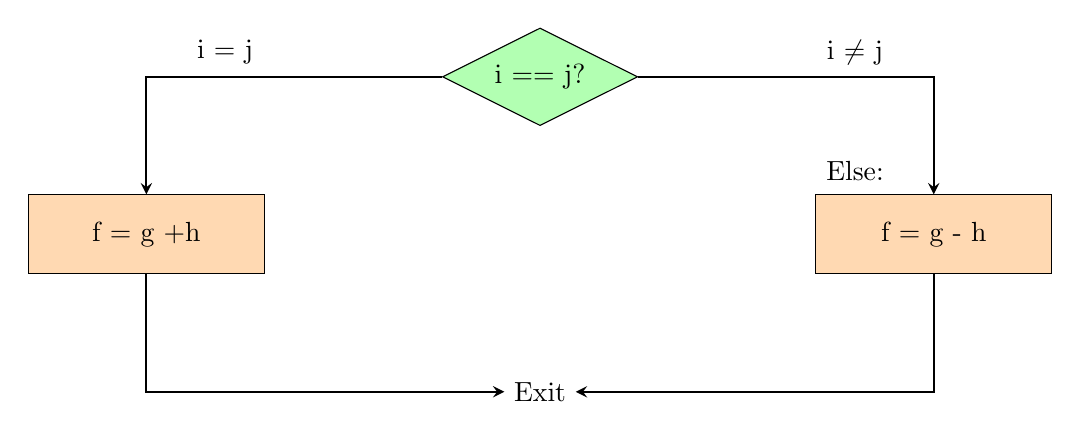
\begin{tikzpicture}[node distance=2cm]
    \node (problem) [decision] {i == j?};
    \node(if)[process, below of=problem, xshift = -5cm]{f = g +h};
    \node(else)[process, below of=problem, xshift = 5cm]{f = g - h};
    \node[above of=else, yshift=-1.2cm, xshift=-1cm]{Else:};
    \node(fine)[below of=if, xshift = 5cm]{Exit};
    \draw [arrow] (problem) -|node[anchor = north, yshift = 0.6cm, xshift = 1cm]{i = j} (if);
    \draw [arrow] (problem) -|node[anchor = north, yshift = 0.6cm, xshift = -1cm]{i \(\not=\) j} (else); 
    \draw [arrow] (if) |- (fine);
    \draw [arrow] (else) |- (fine);
\end{tikzpicture}
\end{center}
Come si vede dal diagramma di flusso viene controllata l'uguaglianza e ci si sposta verso l'istruzione desiderata. Il compilatore per essere più rapido controllerà soltanto che i valori siano discordanti. In questo caso si suppongano tutte le variabili già assegnate ai registri.
\begin{verbatim}
          bne x22, x23, Else      // Vai a Else se i ≠ j
          add x19,x20, x21        // f = g + h (viene saltato se i ≠ j)
          beq x0, x0, Exit        // se 0 == 0 va a Exit (sempre vera)
    Else: sub x19, x20, x21       // f = g - h (viene saltato se i = j)
    Exit: 
\end{verbatim}
Poiché nella loro struttura più basica sono degli \textit{if-else}, anche i \textit{loop} vengono compilati in maniera simile. Il codice in C 
\begin{verbatim}
    while (save[i] == k)\{i += 1\}
\end{verbatim}
viene compilato come (assumendo che \code{i} e \code{k} siano salvati nei registri \code{x22} e \code{x24}, mentre la base dell'array \code{save} sia salvata nel registro \code{x25})
\begin{verbatim}
    Loop: slli x10, x22, 3    // Salva in x10 = i * 8
          add x10, x10, x25   // Salva in x10 l'indirizzo save[i]
          ld x9, 0(x10)       // Salva in x9 il valore di save[i]
          bne x9, x24, Exit   // Va a Exit se x9 ≠ x24 
          addi x22, x22, 1    // Aggiunge 1 a x22
          beq x0, x0, Loop    // Torna a Loop
    Exit:
\end{verbatim}
Un blocco di codice che non si sposta in altre \textit{branch} e non ha \textit{branch} al suo interno è detto blocco base.  
Altri operatori condizionali possono essere per verificare il minore tra due valori \code{blt}, o il maggiore/uguale \code{bge}.

Le operazioni di confronto devono tenere conto della presenza di numeri \textit{signed} e \textit{unsigned}, in quanto un numero con un \(1\) all'inizio può essere un numero molto grande o un numero negativo. Per ovviare a questo problema si utilizzano dei comandi apposta
\begin{center}
    \begin{tabular}{|c|c|c|}
        \hline
        Operatore & Signed & Unsigned \\
        \hline
        = & \code{beq} & \code{beq} \\
        ≠ & \code{bne} & \code{bne} \\
        \(<\) & \code{blt} & \code{bltu} \\
        \(\geq\) & \code{bge} & \code{bgeu} \\
        \hline
    \end{tabular}
\end{center}
\subsection{Programmazione procedurale}
Si definisce programmazione procedurale quella tecnica di suddividere il codice in blocchi più semplici che eseguono sempre lo stesso compito. Si possono definire procedure o \textit{funzioni}. 
In maniera astratta, affinché un programma possa avere una funzione al suo interno deve eseguire sei step
\begin{enumerate}
    \item Salvare i parametri dove la funzione possa accedere
    \item Lasciare il controllo alla funzione
    \item Creare lo spazio in memoria necessario per l'esecuzione
    \item Eseguire il compito
    \item Salvare il risultato dove il programma possa leggerlo
    \item Tornare al punto di origine, così che si possa accedere anche da altri punti del programma
\end{enumerate}
Poiché i registri sono i posti dove è più rapido accedere ai valori, nel RISC-V ci sono \(8\) registri dedicati al salvataggio dei parametri di una procedura (\code{x10-x17}) e \(1\) per tornare al punto di origine \code{x1}.
Un esempio di codice è
\begin{verbatim}
    jal x1, ProcedureAddress  // Si sposta a ProcedureAddress e salva in x1 
                                 l'indirizzo di ritorno
\end{verbatim}
in cui si utilizza il comando \textit{jump-and-link} \code{jal}, che permette di spostarsi in un nuovo indirizzo, salvando l'indirizzo di ritorno della funzione in \code{x1}.
Il ritorno dalla funzione si esegue con il comando \textit{jump-and-link register} \code{jalr}, a cui si assegna il registro \(0\) e si somma il registro \code{x1}
\begin{verbatim}
    jalr x0, 0(x1)            // Si assegna x0 perché non può essere cambiato
\end{verbatim}
Nel caso servano più registri per eseguire un determinato comando, torna utile lo \textit{stack}, una coda che funziona secondo il principio \textit{last-in first-out} (LIFO). Il registro dedicato allo stack è il registro \code{x2}, detto anche \code{sp}.
Prendendo una funzione in C chiamata \code{leaf\_example}
\begin{verbatim}
    long long int leaf_example(long long int g, long long int h, 
                               long long int i, long long int j)
    {
        long long int f;
        f = (g + h) - (i + j);
        return f;
    }
\end{verbatim}
che in RISC-V viene compilata come
\begin{verbatim}
    addi sp, sp, -24    // libera 3 posizioni nello stack
    sd x5, 16(sp)       // salva il registro x5 nello stack
    sd x6, 8(sp)        // salva il registro x6 nello stack
    sd x20, 0(sp)       // salva il registro x20 nello stack
    add x5, x10, x11    // salva in x5 g + h
    add x6, x12, x13    // salva in x6 i + j
    sub x20, x5, x6     // f = x5 - x6 
    addi x10, x20 0     // restituisce f (x10 = x20 + 0)
    ld x20, 0(sp)       // recupera il registro x20 dallo stack
    ld x6, 8(sp)        // recupera il registro x6 dallo stack
    ld x5, 16(sp)       // recupera il registro x5 dallo stack
    addi sp, sp, 24     // toglie le tre posizioni libere dallo stack
    jalr x0, 0(x1)      // torna all'inizio della funzione
\end{verbatim}
I registri \code{x5-x7} e \code{x28-x31} non vengono salvati all'uscita dalla funzione, mentre i registri \code{x8-x9} e \code{x18-x27} rimangono salvati dopo l'esecuzione della funzione.

La funzione sopra viene chiamata \textit{leaf}, perché non richiama altre funzioni.
Quelle che chiamano altre funzioni sono dette \textit{non-leaf}\footnote{Con grande fantasia}. 
Un esempio può essere questa funzione che calcola il fattoriale di un numero
\begin{verbatim}
    long long int fact(long long int n)
    {
        if (n < 1) return(1);
        else return (n * fact(n-1));
    }
\end{verbatim}
che, data in pasto al compilatore, diventa
\begin{verbatim}
    fact:
        addi sp, sp, -16      // libera due elementi nello stack
        sd x1, 8(sp)          // salva x1 nello stack
        sd x10, 0(sp)         // salva x10 nello stack
        addi x5, x10, -1      // x5 = n - 1
        bge x5, x0, L1        // se (n - 1) >= 0, va a L1
        addi x10, x0, 1       // restituisce 1
        addi sp, sp, 16       // riporta lo stack alla situazione iniziale
        jalr x0, 0(x1)        // ritorna
         alla chiamata della funzione 
    L1: 
        addi x10, x10, -1     // n = n -1
        jal x1, fact          // chiama fact(n-1)
        addi x6, x10, 0       // salva il risultato di fact(n-1) in x6
        ld x10, 0(sp)         // recupera il valore n
        ld x1, 8(sp)          // recupera l'indirizzo di ritorno
        mul x10, x10, x6      // n = n* fact(n-1)
        jalr x0, 0(x1)        // torna alla chiamata della funzione
    \end{verbatim}
Una variabile in C può essere salvata in due modi, automatico o statico. Una variabile automatica è accessibile solo da una determinata funzione e viene scartata quando la funzione termina, mentre le variabili statiche sono salvate in memoria e sono accessibili all'esterno e all'interno delle funzioni. Il registro \code{x3} facilita questo compito, creando un \textit{global pointer} \code{gp}, che permette di accedere a tutte le variabili.
\begin{center}
    \begin{tabular}{|c|c|}
        \hline
        Salvati & Temporanei \\
        \hline
        Registri salvati: \code{x8-x9}, \code{x18-x27} & Registri temporanei: \code{x5-x7}, \code{x28, x31} \\
        Stack pointer: \code{x2 (sp)} & \\
        Frame pointer: \code{x8 (fp)} & \\
        Return address: \code{x1 (ra)} & \\
        Stack sopra a \code{sp} & Stack sotto a \code{sp} \\
        \hline
    \end{tabular}
\end{center}
Poiché può capitare che, durante l'esecuzione di una funzione, il valore dello stack pointer cambi, è comodo salvare l'indirizzo iniziale dello stack nel \textit{frame pointer} \code{fp}.

Nel caso di variabili dinamiche, come possono essere le liste, esiste uno spazio di memoria apposito, detto \textit{heap}, dove possono venire salvate ed eventualmente modificate. 
\begin{center}
    \begin{tabular}{|l|c|l|c|}
        \hline
        Nome & Registro & \multicolumn{1}{|c|}{Utilizzo} & Salvato? \\
        \hline
        \code{x0} & 0 & La costante nulla & // \\
        \code{x1 (ra)} & 1 & Indirizzo di ritorno & Sì \\
        \code{x2 (sp)} & 2 & Stack pointer & Sì \\
        \code{x3 (gp)} & 3 & Global pointer & Sì \\
        \code{x4 (tp)} & 4 & Thread pointer & Sì \\
        \code{x5-x7} & 5-7 & Registri temporanei & No \\
        \code{x8-x9} & 8-9 & Registri salvati & Sì \\
        \code{x10-x17} & 10-17 & Argomenti funzione & No \\
        \code{x18-x27} & 18-27 & Registri salvati & Sì \\
        \code{x28-x31} & 28-31 & Registri temporanei & No \\
        \hline
    \end{tabular}
\end{center}
\subsection{Comunicare con il mondo esterno}
I computer inizialmente eseguivano solo conti, ma con il loro divenire sempre più presenti nella vita delle persone è stato necessario trovare una maniera per processare il testo. Lo standard che si utilizza oggi è detto ASCII (American Standard Code for Information Interchange). Con una serie di sitruzioni si possono estrarre i byte da una doubleword, in questo caso però vanno trattati come numeri \textit{unsigned}. Esistono dei comandi apposta \textit{load byte unsigned} \code{lbu} e \textit{store byte} \code{sb}
\begin{verbatim}
    lbu x12, 0(x10)    // legge il byte dalla sorgente
    sb x12, 0(x11)     // scrive il byte sulla destinazione
\end{verbatim}
Un insieme di byte va a formare una stringa. Nel caso del C la fine di una stringa è segnalata dalla presenza del byte \(0\). 
Per esempio il comando \code{strcpy}, che serve a copiare delle stringhe.
\begin{verbatim}
    void strcpy(char x[], char y[])
    {
        size_t i;
        i = 0;
        while ((x[i] = y[i]) != '\0')
            i += 1;
    }
\end{verbatim}
diventa (assumendo che gli indirizzi base di \code{x} e \code{y} sono salvati in \code{x10} e \code{x11}, mentre \code{i} è salvata in \code{x19})
\begin{verbatim}
    strcpy:
        addi sp, sp, -8       // libera un elemento nello stack
        sd x19, 0(sp)         // sposta x19 in cima allo stack
        add x19, x0, x0       // i = 0
    L1:
        add x6, x19, x10      // x5 = indirizzo di y[i]
        lbu x6, 0(x5)         // x6 = y[i]
        add x7, x19, x11      // x7 = indirizzo di x[i]
        sb x6, 0(x7)          // x[i] = y[i]
        beq x6, x0, L2        // se y[i] == 0, termina
        addi x19, x19, 1      // i = i + 1
        jal x0, L1            // ricomincia il loop
    L2: 
        ld x19, 0(sp)         // recupera il registro x19
        addi sp, sp, 8        // riporta lo stack allo stato iniziale
        jalr x0, 0(x1)        // termina
\end{verbatim}
\subsection{Grandi indirizzi in RISC-V}
Sebbene sia molto comodo mantenere tutte le istruzioni di \(32\) bit, ogni tanto può essere comodo avere costanti o indirizzi più grandi.  
Nel caso degli operandi, generalmente il caso più grande includeva \(12\) bit. L'istruzione \textit{load upper immediate} \code{lui} permette di caricare una costante di \(20\) bit dal bit \(12\) al \(31\) di un registro.  
Le istruzioni che permettono di passare da una branch all'altra sono dette del tipo \textit{SB} e sono formate in questa maniera, spezzettando una costante da 12 bit in tante parti
\begin{center}
    \begin{tabular}{|c|c|c|c|c|c|c|c|}
        \hline
        imm[12] & imm[10:5] & rs2 & rs1 & funct3 & imm[4:1] & imm[11] & opcode \\
        \hline
        \multicolumn{1}{c}{1 bit} & \multicolumn{1}{c}{6 bit} & \multicolumn{1}{c}{5 bit} & \multicolumn{1}{c}{5 bit} &\multicolumn{1}{c}{3 bit} &\multicolumn{1}{c}{4 bit} &
        \multicolumn{1}{c}{1 bit} &
        \multicolumn{1}{c}{7 bit}
    \end{tabular}
\end{center}
L'istruzione \code{jal} è del tipo \textit{UJ}, che utilizza solo un registro di destinazione e una costante da \(20\) bit, così ripartita
\begin{center}
    \begin{tabular}{|c|c|c|c|c|c|}
        \hline 
        imm[20] & imm[10:1] & imm[11] & imm[19:12] & rd & opcode \\
        \hline
        \multicolumn{1}{c}{1 bit} & \multicolumn{1}{c}{10 bit} & \multicolumn{1}{c}{1 bit} & \multicolumn{1}{c}{8 bit} & \multicolumn{1}{c}{5 bit} & 
        \multicolumn{1}{c}{7 bit} 
    \end{tabular}
\end{center}
Ma, se tutti gli indirizzi del programma dovessero stare all'interno della costante si avrebbero al massimo \(2^{20}\) possibili indirizzi, che non sono tantissimi. La soluzione arriva dal dividere il \textit{Program Counter} (\textit{PC}) in due parti
\[
    \mbox{Program Counter} = \mbox{Registro attuale} + \mbox{Branch offset}
\]
In questo modo si hanno un totale di \(2^{64}\) indirizzi disponibili per il programma, ma è raro spostarsi di così tanti indirizzi con un cambio di branch o un \code{jal}. Per spostarsi di parecchi indirizzi è necessario usare due istruzioni \code{lui} per scrivere i primi \(20\) bit dell'indirizzo e \code{jalr} per i restanti \(12\).  
Ci sono quindi svariati modi per gestire gli indirizzi 
\begin{enumerate}
    \item Immediate addressing: in questo caso uno degli operandi è una costante che rappresenta l'indirizzo stesso.
    \item Register addressing: in questo caso il registro dell'operazione rappresenta l'indirizzo
    \item Base addressing: in questo caso l'indirizzo si ottiene dalla somma di un registro presente nell'istruzione e una costante
    \item PC-relative addressing: l'indirizzo è ottenuto dalla somma del program counter e una costante presente nell'istruzione
\end{enumerate}
\subsection{Sincronizzazione}
L'esecuzione parallela di vari task è più semplice nel caso siano indipendenti tra di loro, ma non è sempre il caso, anzi, spesso è necessario sincronizzare tra di loro le varie istruzioni. 
Nel caso del RISC-V le istruzioni sono \code{lr.d} (load-reserved doubleword) e \code{sc.d} (store-conditional doubleword). Queste istruzioni vengono usate in sequenza: se la memoria riservata dal primo comando viene modificata prima dell'esecuzione del secondo comando, quest'ultimo non viene eseguito. Infatti \code{sc.d} utilizza tre registri, uno per l'indirizzo, uno per verificare che l'operazione sia andata a buon fine e nell'ultimo il valore da sovrascrivere. Un esempio è dato da 
\begin{verbatim}
    again: lr.d x10, (x20)           // riserva il registro x20
           sc.d x11, x23, (x20)      // salva il valore di x23 in x20
           bne x11, x0, again        // verifica che x11 sia nullo
           addi x23, x10, 0          // salva il valore di x10 in x23
\end{verbatim}
Alla fine di queste linee di codice il valore presente in \code{x23} si trova all'indirizzo di \code{x20} e l'indirizzo di \code{x20} viene salvato in \code{x23}. Il registro \code{x11} viene usato nel caso in cui il registro \code{x20} venga toccato prima che \code{sc.d} possa agire. In tal caso salverà un valore non nullo in \code{x11} che causa il loop del codice finché niente interferisce tra i due comandi.  
\subsection{Tradurre un programma}
Per eseguire un programma sono necessari quattro step fondamentali:
\begin{enumerate}
    \item Compiler: il compilatore prende il programma in C e lo traduce in linguaggio assembly, che è lo step intermedio tra quello che può leggere un umano e quello che può leggere una macchina. Dal linguaggio assembly è necessario passare solo al codice binario affinché la macchina possa leggerlo.
    \item Assembler: alcune istruzioni all'interno del RISC-V sono delle \textit{pseudoistruzioni}, che l'assembler traduce in linguaggio macchina che possa essere effettivamente compreso. Un esempio è l'istruzione \code{li} (load-immediate), che si utilizza come 
    \begin{verbatim}
        li x9, x123
    \end{verbatim}
    che inserisce il valore di \code{x123} in \code{x9}, e viene tradotto come \code{addi} 
    \begin{verbatim}
        addi x9, x0, x123
    \end{verbatim}
    Il compito dell'assembler è quello di produrre un file che è una combinazione di istruzioni in linguaggio macchina, dati e le informazioni necessarie per mantenere tutti i dati al posto giusto.  
    Nel caso dei sistemi UNIX, l'\textit{object-file} è composto da sei parti
    \begin{enumerate}
        \item[I.] l'header, che descrive la dimensione e la posizione di tutti gli altri pezzi dentro il file
        \item[II.] il \textit{text segment} che contiene tutta la parte di linguaggio macchina
        \item[III.] il \textit{static data segment} contiene tutti i dati necessari per l'esecuzione del programma (nei sistemi UNIX sono presenti anche i dati dinamici)
        \item[IV.] la \textit{relocation information} identifica le istruzioni e i dati che dipendono da indirizzi assoluti quando il programma viene caricato in memoria
        \item[V.] la \textit{symbol table} contiene le \textit{label} che non sono ancora state definite 
        \item[VI.] la \textit{debugging information} che descrive come sono stati compilati i vari moduli  
    \end{enumerate}
    \item Linker: finora si è sempre parlato di compilare il programma riga per riga ogni volta che veniva eseguito. Dal momento che questa pratica richiede una quantità esagerata di risorse, si utilizza allora un comodo strumento che compila indipendentemente tutte le linee di codic e e le unisce alla fine, in tal modo, se viene modificata una sola linea, tutte le altre saranno già compilate. Una volta fatto questo si occupa di verificare tutte le referenze interne ed esterne al programma e assegnare ad esse i corretti indirizzi in memoria. Una volta fatto questo viene prodotto un \textit{file eseguibile} che può essere fatto girare sulla macchina
    \item Loader: una volta creato l'\textit{eseguibile}, nei sistemi UNIX avvengono sei step
    \begin{enumerate}
        \item viene letto l'header del file per calcolare la dimensione del \textit{text segment} e \textit{data segment}
        \item viene creato abbastanza spazio negli indirizzi per il testo e i dati
        \item vengono copiate le istruzioni e i dati dal file alla memoria
        \item vengono copiati eventuali parametri dal main allo stack
        \item vengono inizializzati i registri del processore e posizionato lo stack pointer
        \item si entra in una branch di start up che copia i parametri dallo stack ai registri degli argomenti e chiama il main del programma. Quando il main si chiude, lo start up esce dall'esecuzione del programma
    \end{enumerate}
\end{enumerate}
Le librerie venivano utilizzate in modo statico inizialmente, ma questo portava ad alcuni svantaggi
\begin{itemize}
    \item la libreria faceva parte del codice eseguibile, per cui se questa veniva aggiornata, andava aggiornata anche dentro il codice, che altrimenti continuava a recuperare la versione vecchia
    \item vengono caricate tutte le funzioni all'interno della libreria anche se non vengono poi utilizzate, che spesso significa un grande spreco di memoria
\end{itemize}
Questi svantaggi hanno portato allo sviluppo delle \textit{dynamically linked libraries} (DLLs) che vengono chiamate dal programma nel momento dell'esecuzione in maniera dinamica, evitando di recuperare versioni obsolete e di saturare la memoria chiamando tutte le librerie non necessarie.  
\subsection{Un esempio in C}
In questa sezione si cerca di fare un riassunto di quanto visto finora, partendo da due snippet di codice in C
\begin{verbatim}
    void swap(long long v[], size_t  k)
    {
        long long temp;
        temp = v[k];
        v[k] = v[k+1];
        v[k+1] = temp;
    }
\end{verbatim}
Questo codice prende un elemento in un array e lo scambia con un altro elemento dell'array, modificando solo le loro posizioni. Per tradurlo in linguaggio macchina è necessario seguire tre step
\begin{itemize}
    \item Allocare i registri per le variabili del programma
    \item Creare il codice per la funzione 
    \item Mantenere inalterati i registri durante le eventuali iterazioni della funzione
\end{itemize}
Per allocare i registri, il RISC-V utilizza convenzionalmente \code{x10-x17} per i parametri della funzione. In questo caso, essendo solo due, si troveranno in \code{x10} e \code{x11}. La variabile interna \code{temp} sarà allocata al registro \code{x5}.  
A questo punto rimangono solo le linee di codice
\begin{verbatim}
    temp = v[k];
    v[k] = v[k+1];
    v[k+1] = temp;
\end{verbatim}
Dal momento che il RISC-V utilizza gli indirizzi in \textit{byte}, ogni doubleword dista da quella prima \(8\) bit, quindi tutti gli indici vanno moltiplicati per \(8\).  

Per ottenere il valore di \code{v[k]} bisogna moltiplicare il valore di \code{k} per \(8\), tramite uno \textit{shift left} di 3
\begin{verbatim}
    slli x6, x11, 3    
\end{verbatim}
che salva in \code{x6} il valore \code{k * 8}
\begin{verbatim}
    add x6, x10, x6
\end{verbatim}
che aggiunge a \code{x6} il valore dell'indirizzo base di \code{v}, in maniera da ottenere \code{v[k]}
\begin{verbatim}
    ld x5, 0(x6)
    ld x7, 8(x6)
\end{verbatim}
in \code{x5} viene salvato il valore \code{v[k]}, e aggiungendo \(8\) bit si ottiene il valore \code{v[k+1]} che viene salvato in \code{x6}
\begin{verbatim}
    sd x7, 0(x6)
    sd x5, 8(x6)
\end{verbatim}
a questo punto vengono caricati \code{v[k+1]} alla posizione di \code{v[k]} e viceversa.  

Riassumendo il tutto, la funzione \code{swap} si traduce in RISC-V come

\begin{verbatim}
    swap:
        slli x6, x11, 3      // reg x6 = k * 8
        add x6, x10, x6      // reg x6 = v + (k * 8)
        ld x5, 0(x6)         // reg x5 (temp) = v[k]
        ld x7, 8(x6)         // reg x7 = v[k+1]
        sd x7, 0(x6)         // v[k] = reg x7
        sd x5, 8(x6)         // v[k+1] = reg x5
        jalr x0, 0(x1)       // return
\end{verbatim}
Un altro esempio è dato dalla funzione \code{sort}, che in questo caso si occupa di mettere in ordine crescente gli elementi di un array. La funzione è scritta come
\begin{verbatim}
    void sort (long long v[], size_t int n)
    {
        size_t i, j;
        for (i = 0; i < n; i += 1) {
            for (j = i - 1; j >= 0 && v[j] > v[j+1]; j -= 1){
                swap(v, j);
            }
        }
    }
\end{verbatim}
Per prima cosa vengono allocati i registri necessari per i parametri della funzione, in questo caso \code{v} sarà associato a \code{x10}, \code{n} a \code{x11}, \code{i} a \code{x19} e \code{j} a \code{x20}.  
La funzione è composta da due \code{for} loop annidati e una chiamata alla funzione \code{swap}. I loop sono composti da tre parti, una inizializzazione di variabile, un test e un incremento.  
Il primo loop è dato sostanzialmente da 
\begin{verbatim}
        li x19, 0            // i  = 0
    for1tst:
        bge x19, x11, exit1  // esce se i >= n
        ...
        eventuali istruzioni del loop
        ... 
        addi x19, x19, 1     // i += 1
        j for1tst            // torna al loop
    exit1:
\end{verbatim}
Il secondo loop è leggermente più complesso 
\begin{verbatim}
        addi x20, x19, -1    // j = i - 1
    for2tst:
        blt x20, x0, exit2   // esce se j < 0
        slli x5, x20, 3      // reg x5 = j * 8
        add x5, x10, x5      // reg x5 = v + (j * 8)
        ld x6, 0(x5)         // reg x6 = v[j]
        ld x7, 8(x5)         // reg x7 = v[j+1]
        ble x6, x7, exit2    // esce se v[j] <= v[j+1]
        ... 
        eventuali istruzioni del loop
        ... 
        addi x20, x20, -1    // j -= 1
        j for2tst            // torna in cima al loop
    exit2:
\end{verbatim}
A questo punto rimane solo l'istruzione che chiama \code{swap}, che di per sé è abbastanza semplice
\begin{verbatim}
    jal x1, swap
\end{verbatim}
Tuttavia rimane il problema di passare i parametri corretti, perché sia \code{sort} che \code{swap} leggono i parametri da \code{x10} e \code{x11}. Un modo per farlo può essere quello di salvare i parametri da un'altra parte prima
\begin{verbatim}
    mv x21, x10               // copia x10 in x21
    mv x22, x11               // copia x11 in x20
\end{verbatim}
Per poi riprenderli quando viene chiamata \code{swap}. 
Inoltre è necessario fare spazio per i registri necessari nello stack a inizio procedura.  
Mettendo assieme tutti i pezzi si ottiene la traduzione in RISC-V della funzione \code{sort}
\begin{verbatim}
    sort:
        addi sp, sp, -40      // libera 5 elementi nello stack
        sd x1, 32(sp)         // salva x1 nello stack 
        sd x22, 24(sp)        // salva x22 nello stack        
        sd x21, 16(sp)        // salva x21 nello stack
        sd x20, 8(sp)         // salva x20 nello stack
        sd x19, 0(sp)         // salva x19 nello stack
        mv x21, x10           // copia x10 in x21
        mv x22, x11           // copia x11 in x22 
        li x19, 0             // i = 0
    for1tst:
        bge x19, x22, exit1   // esce se i >= n
        addi x20, x19, -1     // j = i - 1
    for2tst:
        blt x20, x0, exit2    // esce se j < 0
        slli x5, x20, 3       // reg x5 = j * 8
        add x5, x10, x5       // reg x5 = v + (j * 8)
        ld x6, 0(x5)          // reg x6 = v[j]
        ld x7, 8(x5)          // reg x7 = v[j+1]
        ble x6, x7, exit2     // esce se v[j] <= v[j+1]
        mv x10, x21           // recupera v dallo stack in x10
        mv x11, x22           // recupera j dallo stack in x11
        jal x1, swap          // chiama swap
        addi x20, x20, -1     // j -= 1
        j for2tst             // torna a for2tst
    exit2:
        addi x19, x19, 1      // i += 1
        j for1tst             // torna a for1tst
    exit1:
        ld x19, 0(sp)         // recupera x19 dallo stack
        ld x20, 8(sp)         // recupera x20 dallo stack
        ld x21, 16(sp)        // recupera x21 dallo stack
        ld x22, 24(sp)        // recupera x22 dallo stack
        ld x1, 32(sp)         // recupera x1 dallo stack
        addi sp, sp, 40       // riporta alla posizione iniziale lo stack
        jalr x0, 0(x1)        // esce dalla funzione
\end{verbatim}
\subsection{Array e puntatori}
Ogni persona che si affaccia alla programmazione in C deve affrontare l'annosa questione dei puntatori. In questo caso si prendono a esempio due funzioni che, dato un array in ingresso, lo restituisce contenente solo valori nulli. 
\begin{center}
    \begin{tabular}{|p{8cm}|p{8cm}|}
    \hline
    Indici & Puntatori \\
    \hline
        \begin{verbatim}
clearindices(long long array[],
            size_t int size)
{
    size_t i;
    for (i = 0; i < size, i += 1)
            array[i] = 0;
}
        \end{verbatim}
        
        &
        
        \begin{verbatim}
clearpointers(long long *array[],
             size_t int size)
{
    long long *p;
    for (p = &array[0], 
        p < &array[size], p += 1)
            *p = 0;
}
        \end{verbatim} 
        \\
        \hline
        \begin{verbatim}
    li x5, 0        // i = 0
loop:
    slli x6, x5, 3  // x6 = i * 8
    add x7, x10, x6 // x7 = 
                         indirizzo
                         array[i]
    sd x0, 0(x7)    // array[i] = 0
    addi x5, x5, 1  // i += 1
    blt x5, x11, loop1 
        \end{verbatim}
        &
        \begin{verbatim}
    mv x5, x10      // p = indirizzo
                            array[0]
    slli x6, x11, 3 // Memory[p] = 0
    add x7, x10, x6 // p = p + 8
loop2: 
    sd x0, 0(x5)    // x6 = size * 8
    addi x5, x5, 8  // x7 =indirizzo
                       array[size]
    bltu x5, x7, loop2
    \end{verbatim}
        \\
        \hline
    \end{tabular}
\end{center}
Nel caso degli array tutte le operazioni avvengono all'interno del loop, quindi la variabile \code{i} viene incrementata e ogni indirizzo va calcolato nuovamente. Nel secondo caso l'incremento avviene direttamente sull'indirizzo, riducendo il numero di operazioni. Al giorno d'oggi i compilatori riescono comunque ad ottimizzare la versione con gli array a un livello pari a quella con i puntatori, per cui non vi è grande differenza nell'utilizzo. 
\newpage
\section{Aritmetica dei calcolatori}
\subsection{Introduzione}
Come visto in precedenza, tutto nei computer è composto da bit. A questo punto sorge spontaneo chiedersi cosa succeda per tutti gli altri numeri? Come vengono rappresentati i numeri reali? Se si cerca di calcolare un numero più grande di quelli che può rappresentare il computer? Come funzionano moltiplicazioni e sottrazioni? 

Tutte queste domande sono legate al funzionamento dell'aritmetica dei calcolatori, il cui funzionamento verrà spiegato in questa sezione.
\subsection{Addizioni e sottrazioni}
Il funzionamento delle addizioni in un computer è abbastanza semplice, si sommano i numeri e eventuali riporti vengono spostati a sinistra. Un esempio possono essere i numeri \(6_{\mbox{\scriptsize dieci}} \mbox{ e } 7_{\mbox{\scriptsize dieci}}\).
\[
\begin{array}{cccc}
    & 00000111_{\mbox{\scriptsize due}} & = & 7_{\mbox{\scriptsize dieci}} \\
    + & 00000110_{\mbox{\scriptsize due}} & = & 6_{\mbox{\scriptsize dieci}} \\
    \hline
    = & 00001101_{\mbox{\scriptsize due}} & = & 13_{\mbox{\scriptsize dieci}}
\end{array}    
\]
Nel caso della sottrazione si somma il negativo del numero da sottrarre, nel caso appena visto si avrà: 
\[
\begin{array}{cccc}
    & 00000111_{\mbox{\scriptsize due}} & = & 7_{\mbox{\scriptsize dieci}} \\
    + & 11111010_{\mbox{\scriptsize due}} & = & -6_{\mbox{\scriptsize dieci}} \\
    \hline
    = & 00000001_{\mbox{\scriptsize due}} & = & 1_{\mbox{\scriptsize dieci}}
\end{array}    
\]
In questo caso si tratta di somme in complemento a due, perché i numeri negativi hanno bisogno di un bit speciale che rappresenti il meno all'inizio. Si hanno quindi un numero limitato di numeri che possono essere rappresentati, dando vita all'\textit{overflow}, ossia quando si eccede il numero di bit possibili e il risultato dell'operazione non è quello atteso.
\begin{center}
\begin{tabular}{|c|c|c|c|}
    \hline
    \multicolumn{4}{|c|}{Quando avviene overflow?} \\
    \hline
    Operazione & Operando A & Operando B & Risultato in caso di overflow \\
    \hline
    A + B & \(\geq\)0 & \(\geq\)0 & \(<\)0 \\
    \hline
    A + B & \(<\)0 & \(\geq\)0 & \(\geq\)0 \\
    \hline
    A - B & \(\geq\)0 & \(<\)0 & \(<\)0 \\
    \hline
    A - B & \(<\)0 & \(\geq\)0 & \(\geq\)0 \\
    \hline
\end{tabular} 
\end{center}
\subsection{Moltiplicazioni}
Per comprendere le moltiplicazioni in base binaria bisogna prima riprendere il concetto di moltiplicazione in base decimale. Si veda la moltiplicazione \(1000_{\mbox{\scriptsize dieci}} \times 1001_{\mbox{\scriptsize dieci}}\)
\begin{center}
    \begin{tabular}{cccccccccc}
        Moltiplicando & & & & & 1 & 0 & 0 & 0 & \(\times\)\\
        Moltiplicatore & & & & & 1 & 0 & 0 & 1 & =\\
        \hline
        & & & & & 1 & 0 & 0 & 0 & +\\
        & & & 0 & 0 & 0 & 0 & & & +\\
        & & 0 & 0 & 0 & 0 & & & & +\\
        & 1 & 0 & 0 & 0 & & & & & =\\
        \hline
        & 1 & 0 & 0 & 0 & 1 & 0 & 0 & 0 &\\
    \end{tabular}
\end{center}
Questo è l'algoritmo classico della moltiplicazione, ristretto al caso delle cifre \(1\) e \(0\). Nel caso al moltiplicatore sia presente un \(1\) viene riscritto il moltiplicando partendo dalla posizione dell'\(1\). In caso si abbia uno \(0\) si riscrive semplicemente \(0\). 
Nel caso del computer si prende come esempio questo classico algoritmo e si ottimizza per l'hardware presente. Si assuma che il moltiplicatore sia una parola da 64-bit e che il prodotto sia una parola da 128-bit in un registro inizializzato a 0. Durante l'algoritmo il moltiplicatore subisce un bit shift verso destra per 64 volte, per riempire tutti i bit del prodotto. Allora segue che anche il moltiplicando sarà una parola da 128-bit.  

Sostanzialmente l'algoritmo fa un check per vedere se l'ultima cifra del moltiplicatore è uno 0 o un 1 e a seconda del risultato somma al prodotto 0 o il valore del moltiplicando, fatto questo, fa uno shift verso sinistra del moltiplicando e uno shift verso destra del moltiplicatore, per poi ripetere tutto. 
\begin{center}
    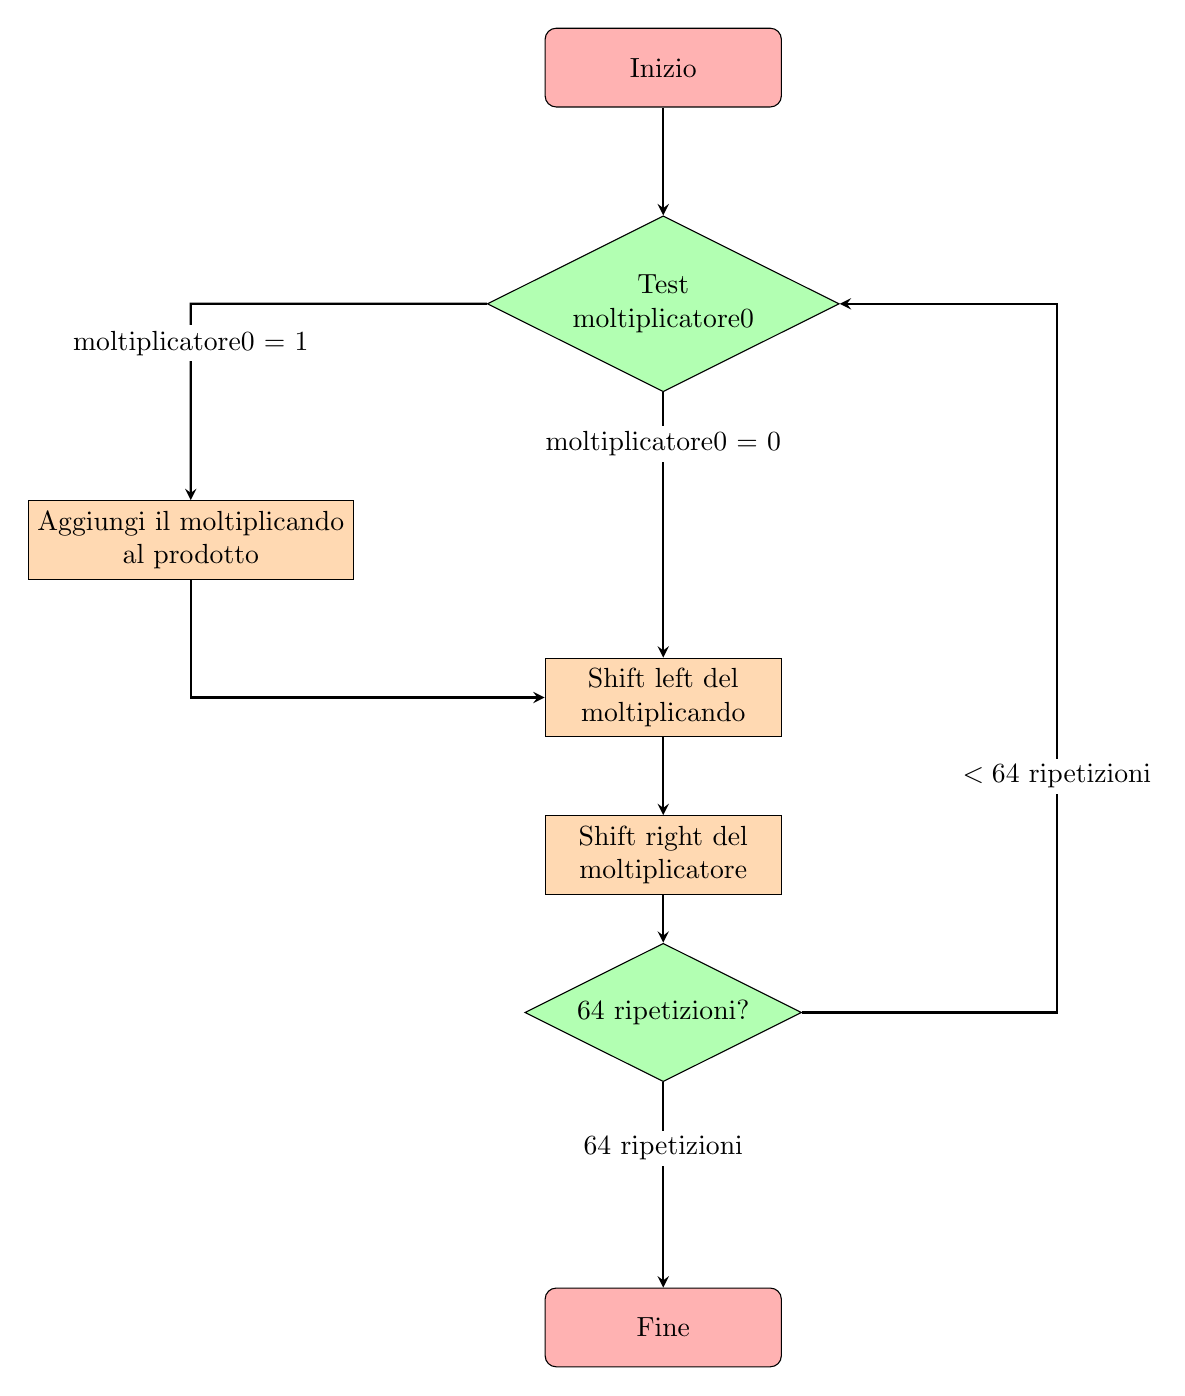
\begin{tikzpicture}[node distance=2cm]
        \node (inizio) [startstop] {Inizio};
        \node (problem) [decision, below of= inizio, align=center, yshift=-1cm] {Test\\ moltiplicatore0};
        \node(if)[process, below of=problem, xshift = -6cm, yshift = -1cm,align=center]{Aggiungi il moltiplicando\\
        al prodotto};
        \node (shiftleft) [process, below of= if, align= center, xshift= 6cm] {Shift left del\\ 
        moltiplicando};
        \node (shiftright) [process, below of= shiftleft, align=center]{Shift right del \\ 
        moltiplicatore};
        \node (ripetizioni) [decision, below of=shiftright, align=center]{64 ripetizioni?};
        \node(fine)[startstop, below of=ripetizioni, yshift=-2cm]{Fine};
        \draw [arrow] (problem) -|node[pos=0.75,fill=white,inner sep=2pt]{moltiplicatore0 = 1} ++(-6,-1) --(if);
        \draw [arrow] (problem) --node[pos=0.75,fill=white,inner sep=2pt]{moltiplicatore0 = 0} ++(0,-2) --(shiftleft);
        \draw [arrow] (ripetizioni) -|node[pos=0.75,fill=white,inner sep=2pt]{\(<64\) ripetizioni} ++(5,6) |-(problem);
        \draw [arrow] (inizio) -- (problem);
        \draw [arrow] (if)|-(shiftleft);
        \draw [arrow] (shiftleft)--(shiftright);
        \draw [arrow] (shiftright) --(ripetizioni);
        \draw [arrow] (ripetizioni)--node[pos=0.75,fill=white,inner sep=2pt]{64 ripetizioni} ++(0,-2)--(fine);
    \end{tikzpicture}
    \end{center}
Chiaramente questo algoritmo si può parallelizzare per migliorarne l'efficienza, ad esempio ricreando il diagramma sopra in modo che non esegua una somma alla volta, ma lavori in parallelo per tutte le 64 somme.
\subsection{Divisione}
L'opposto della motliplicazione è la divisione, che è una operazione ancora più complicata da gestire, ad esempio perché non si può dividere per 0.

Come per la moltiplicazione, un esempio di divisione tra due numeri in base 10
\begin{center}
    \begin{tabular}{cccc}
        & & \multicolumn{1}{r}{$1001_{\mbox{\scriptsize dieci}}$} & Quoziente \\
        \hhline{~~-~}
        Divisore & \(1000_{\mbox{\scriptsize dieci}}\) & \multicolumn{1}{|r}{\phantom{-}\(1001010_{\mbox{\scriptsize dieci}}\)} & Dividendo \\
        & & \multicolumn{1}{l}{-1000} & \\
        \hhline{~~-~}
        & & \multicolumn{1}{l}{\phantom{10}10} & \\
        & & \multicolumn{1}{l}{\phantom{10}101} & \\
        & & \multicolumn{1}{l}{\phantom{10}1010} & \\
        & & \multicolumn{1}{l}{\phantom{10}-1000} & \\
        \hhline{~~-~}
        & & \phantom{1000}\(10_{\mbox{\scriptsize dieci}}\) & Resto \\
    \end{tabular}
\end{center}
\[
\mbox{Dividendo} = \mbox{Quoziente} \times \mbox{Divisore} + \mbox{Resto}    
\]
\begin{center}
    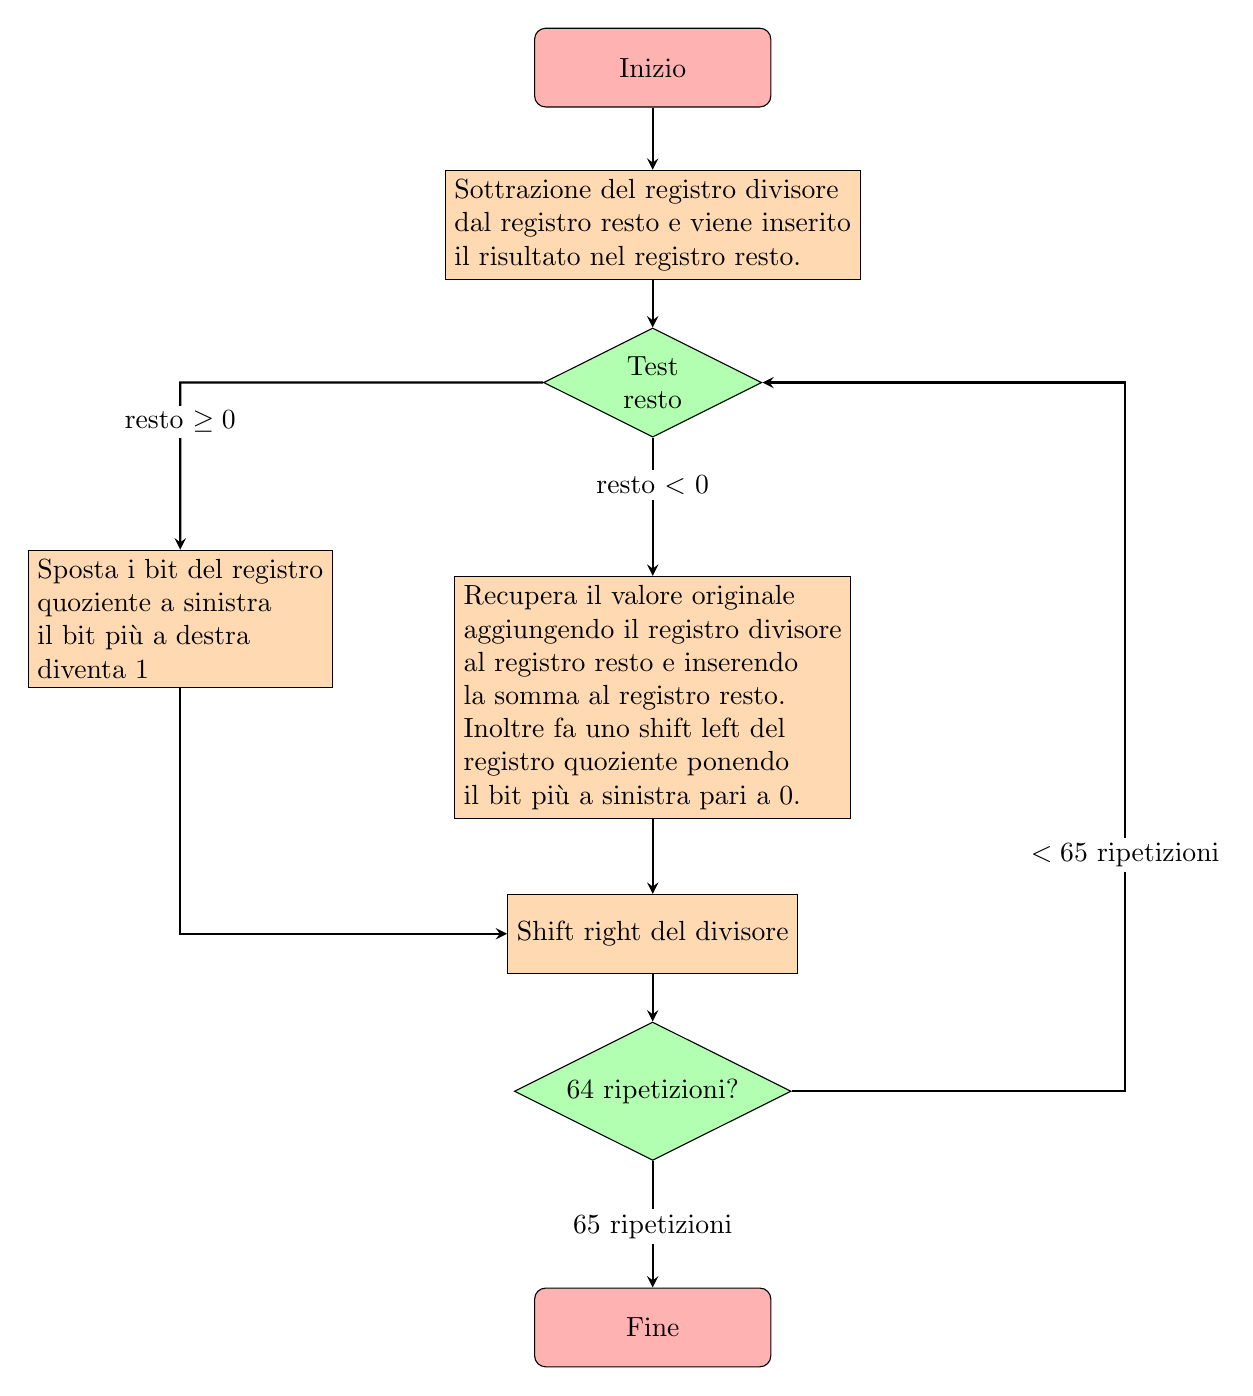
\begin{tikzpicture}[node distance=2cm]
        \node (inizio) [startstop] {Inizio};
        \node (primaop) [process, below of = inizio, align = left] {Sottrazione del registro divisore \\
        dal registro resto e viene inserito\\ 
        il risultato nel registro resto.};
        \node (problem) [decision, below of= primaop, align=center] {Test\\ resto};
        \node(if)[process, below of=problem, xshift = -6cm, yshift = -1cm,align=left]{Sposta i bit del registro \\ 
        quoziente a sinistra\\ 
        il bit più a destra \\ 
        diventa 1};
        \node (else)[process, below of = problem, align = left,yshift = -2cm] {Recupera il valore originale \\ 
        aggiungendo il registro divisore \\ 
        al registro resto e inserendo \\ 
        la somma al registro resto. \\ 
        Inoltre fa uno shift left del \\ 
        registro quoziente ponendo \\ 
        il bit più a sinistra pari a 0.};
        \node (shiftright) [process, below of= problem,yshift = -5cm, align=center]{Shift right del divisore};
        \node (ripetizioni) [decision, below of=shiftright, align=center]{64 ripetizioni?};
        \node(fine)[startstop, below of=ripetizioni, yshift=-1cm]{Fine};
        \draw [arrow] (problem) -|node[pos=0.75,fill=white,inner sep=2pt]{resto \(\geq 0\)} ++(-6,-1) --(if);
        \draw [arrow] (problem) --node[pos=0.75,fill=white,inner sep=2pt]{resto \(<\) 0} ++(0,-1.5) --(else);
        \draw [arrow] (ripetizioni) -|node[pos=0.75,fill=white,inner sep=2pt]{\(<65\) ripetizioni} ++(6,6) |-(problem);
        \draw [arrow] (inizio) -- (primaop);
        \draw [arrow] (primaop) -- (problem);
        \draw [arrow] (if)|-(shiftright);
        \draw [arrow] (shiftright) --(ripetizioni);
        \draw [arrow] (else) -- (shiftright);
        \draw [arrow] (ripetizioni)--node[pos=0.75,fill=white,inner sep=2pt]{65 ripetizioni} ++(0,-2)--(fine);
    \end{tikzpicture}
    \end{center}
    L'algoritmo sarà sostanzialmente una sottrazione continua del numero più grande che si riesce a sottrarre moltiplicando il divisore, aggiungendo ogni volta una cifra al quoziente, fino ad arrivare a un valore più piccolo del divisore, che sarà il resto.
    Nel caso di una divisione con i \textit{signed integers}, sarà necessaria la presenza di un bit di segno che distingua numeri positivi e negativi.

    Anche in questo caso viene in aiuto la legge di Moore che permette di accelerare questo processo con la tecnica SRT. Con tale tecnica si cerca di predire più bit del quoziente con l'utilizzo di una lookup table, che permette di accelerare il processo se la tabella è usata correttamente.
    \subsection{Floating point}
    Nel mondo reale, tuttavia, non esistono solo i numeri interi, per cui è stato necessario trovare un modo per rappresentare i numeri reali con i computer. Un metodo affermato per rappresentare i numeri in base decimale è la notazione scientifica.
    \[
        3.141592_{\mbox{\scriptsize dieci}} \times 10^9
    \]
    Allo stesso modo si può usare la notazione scientifica per i numeri in base binaria
    \[
        1.0_{\mbox{\scriptsize due}} \times 2_{-1}
    \]
    In questo modo si può rappresentare un numero con al suo interno una virgola che si sposta al variare dell'esponente della base 2. Questa notazione è detta \textit{floating point} (virgola mobile per quelli a cui piace dire calcolatore), la cui forma sarà quindi 
    \[
        1.xxxxxxxx_{\mbox{\scriptsize due}} \times 2^{yyyy}    
    \]
    In questo caso si è tenuto per semplicità l'esponente in base decimale, ma chiaramente si tratta di un numero in base binaria.
    È necessario trovare un compromesso tra la dimensione della frazione e quella dell'esponente, ricordando che i registri all'interno del RISC-V sono di 32 bit. Il consenso si è raggiunto nel creare un numero della forma 
    \[
        (-1)^S \times F \times 2^E
    \]
    \begin{center}
        \begin{tabular}{|c|c|c|}
            \hline
            s & esponente & frazione \\
            \hline
            \multicolumn{1}{c}{\normalsize 1 bit} & \multicolumn{1}{c}{\normalsize 8 bit} & \multicolumn{1}{c}{\normalsize 23 bit}        
        \end{tabular}
    \end{center}
    In questa maniera è abbastanza facile ottenere numeri molto precisi, con tante cifre dopo la virgola, ma anche numeri molto grandi, senza nessun numero dopo la virgola. Nel caso il numero da rappresentare sia troppo piccolo per le capacità del registro si parla di \textit{underflow}.
    Per ovviare a questo problema si utilizzano due differenti tipi di numeri floating point. Quello appena visto è detto \textit{single precision} ed è formato da 32 bit, mentre l'altro è detto \textit{double precision} ed è formato da 64 bit, di cui 52 per la frazione e 11 per l'esponente. 

    Nel caso dei numeri floating point l'addizione è costituita da una serie di passaggi:
    \begin{itemize}
        \item[Step 1.] Per sommare due numeri in notazione scientifica è necessario allineare i due numeri in modo che le cifre dopo la virgola siano le stesse, per esempio \( 9.999_{\mbox{\scriptsize dieci}} \times 10^1\) e \(1.610_{\mbox{\scriptsize dieci}} \times 10^{-1}\) 
        \[
            1.610_{\mbox{\scriptsize dieci}} \times 10^{-1} = 0.1610_{\mbox{\scriptsize dieci}} \times 10^0 = 0.01610 \times 10^1
        \]
        \item[Step 2.] Poi c'è l'addizione delle due frazioni \[9.999_{\mbox{\scriptsize dieci}} \times 10^1 + 0.016_{\mbox{\scriptsize dieci}} \times 10^1 = 10.015_{\mbox{\scriptsize dieci}} \times 10^1\]
        \item[Step 3.] A questo punto va normalizzato il risultato \[10.015_{\mbox{\scriptsize dieci}} \times 10^1 = 1.0015_{\mbox{\scriptsize dieci}}\times 10^2\]  
        \item[Step 4.] Siccome i due numeri avevano quattro cifre significative, va arrotondato questo numero ottenuto al numero corretto di cifre significative
        \[
           1.0015_{\mbox{\scriptsize dieci}} \times 10^2 = 1.002_{\mbox{\scriptsize dieci}} \times 10^2 
        \] 
    \end{itemize}
In maniera simile si affronta la moltiplicazione tra numeri floating-point. Si prendano i numeri \(1.110_{\mbox{\scriptsize dieci}} \times 10^{10} \times 9.200_{\mbox{\scriptsize dieci}} \times 10^(-5)\).
\begin{itemize}
    \item[Step 1.] Per prima cosa si ottiene l'esponene del prodotto con la somma degli esponendi dei due fattori  
    \[
        10 + (-5) = 5
    \] 
    \item[Step 2.] A questo punto è necessario eseguire la moltiplicazione dei due fattori 
    \[1.110_{\mbox{\scriptsize dieci}} \times 9.200_{\mbox{\scriptsize dieci}} = 10.212000_{\mbox{\scriptsize dieci}}\]
     che quindi diventa \(10.212_{\mbox{\scriptsize dieci}} \times 10^5\)
    \item[Step 3.] Lo step successivo, come nell'addizione è la normalizzazione e eventuale arrotondamento, ossia
    \[
        10.212_{\mbox{\scriptsize dieci}} \times 10^5 = 1.0212_{\mbox{\scriptsize dieci}} \times 10^6
    \]  
    che chiaramente diventa \(1.021_{\mbox{\scriptsize dieci}} \times 10^6\)
    \item[Step 4.] Lo step finale è la verifica dei bit di segno dei due fattori per stabilire il segno del risultato.
\end{itemize}
A seguire un piccolo snippet di codice utilizzato per convertire la temperatura da gradi Celsius a gradi Fahrenheit.
\begin{verbatim}
    float f2c (float fahr){
        return ((5.0f/9.0f) * (fahr - 32.0f));
    }
\end{verbatim}
diventa in RISC-V 
\begin{verbatim}
    f2c:
        flw f0, const5(x3)   // f0 = 5.0f
        flw f1, const9(x3)   // f1 = 9.0f
        fdiv.s f0, f0, f1    // f0 = 5.0f/9.0f
        flw f1, const32(x3)  // f1 = 32.0f
        fsub.s f10, f10, f1  // f10 = fahr - 32.0f
        fmul.s f10, f0, f10  // f10 = (5.0f /9.0f) * (fahr - 32.0f)
        jalr x0, 0(x1)       // return
\end{verbatim}
\section{Il processore}
\subsection{Le regole logiche}
Bisogna stabilire delle convenzioni da seguire 
\end{document}
